\section{Diseño de los flits y paquetes}

Llamamos \textit{flit} a cada una de las unidades lógicas mínimas que podemos enviar por la red. Un paquete está formado por varios \textit{flits}, donde el primero de ellos solo tiene información relevante para los conmutadores y llamamos \textit{cabecera}, y el último se encarga de cerrar la conexión y se denomina \textit{cola} (figura \ref{fig:packets}). Mandamos los flits de manera secuencial para formar un paquete, sin embargo, el envío de cada uno de los flits individuales puede realizarse tanto de manera secuencial (segmentada) como en paralelo con un bus del tamaño del flit.

\begin{figure}[h]
    \centering
    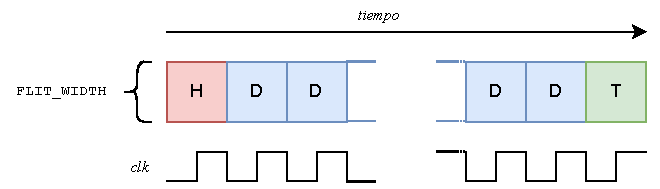
\includegraphics{images/diagrams/packets.drawio.pdf}
    \caption{Diagrama temporal del envío de un paquete completo a lo largo de la red.}
    \label{fig:packets}
\end{figure}

Una alternativa al sistema de \textit{flit de cola} es especificar el tamaño del paquete en la cabecera. Sin embargo, esta solución requiere de aumentar el tamaño de la cabecera y restringe el tamaño máximo de un paquete.

En caso de querer enviar un paquete de un tamaño en bits que no sea múltiplo del ancho del flit, es necesario comunicar de alguna manera el tamaño en bits del paquete para poder ignorar los sobrantes. Por ejemplo, especificándolo en los bits libres de la cabecera, o fijándolo en el protocolo si el tamaño es invariable y conocido de antemano.

\begin{recuadronoc}
    En nuestra NoC, cada \textit{flit} se manda en paralelo por un bus de tamaño \textit{FLIT\_WIDTH} para evitar crear más dominios de reloj y simplificar el diseño. En caso de enviar los bits en serie se necesitaría una frecuencia de reloj demasiado alta (aumentando el consumo dinámico), mientras que añadir pistas al diseño no supone un problema.

    El flit cabecera contiene simplemente la información de destino del paquete, y los flits de datos y cola tienen casi todo el espacio libre. Puede verse de manera detallada la codificación de los flits en la subsección \ref{subsec:codificacion_flits}
\end{recuadronoc}
